% !TeX root = ../main.tex
% Add the above to each chapter to make compiling the PDF easier in some editors.

\chapter{Methods}\label{chapter:methods}

In this paper, developers’ quality was evaluated using the SZZ algorithm \parencite{Sliwerski} and the programmers were divided into two groups—\textit{good} and \textit{bad}. The focus of both groups was examined for comparison. Focus was measured based on the extensions that developers worked on. \par

\begin{figure}[htpb]
  \centering
  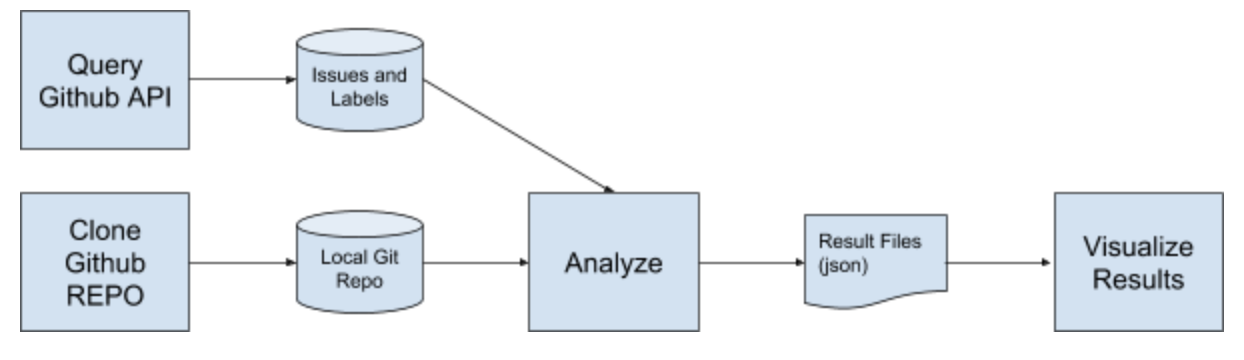
\includegraphics[width=0.8\textwidth]{figures/process}
  \caption[The Process]{The diagram displays the process followed in this research. The data is gathered via combination of GitHub API and locally cloned repositories. Using the data, good developers are selected and the focus of all the authors is analyzed. The results are saved in a form of JSON files for further visualization and analysis.} \label{fig:process}
\end{figure}

\section{Data Set}

The data was extracted from GitHub using a time-filter of four years— from beginning of 2014 until the end of 2017. Over 200,000 commits were collected from ten repositories that contained over 3,000 contributors across seven major languages. The selected repositories included: \par

\begin{itemize}
  \item Elasticsearch
  \item Ansible
  \item Servo
  \item Bitcoin
  \item Selenium
  \item Spring-boot
  \item Rust
  \item TypeScript 
  \item Symfony
  \item Rails
\end{itemize}

The issues and the labels were downloaded via the GitHub API, while the commits and further processing was done utilizing additional information obtained by locally cloning the repositories and executing Git commands. The processing is described in detail under Good Developer and Focus Analysis subsections. 

\section{Repository Selection}

Because a majority of GitHub repositories is personal and not related to coding\parencite{perils}, the repositories used for the research were carefully selected. The following criteria were used.

\begin{table}[h!]
\begin{center}
\begin{tabular}{ | m{12em} | m{20em}| } 
\hline
Characteristic & Criteria \\ 
\hline \hline
Age & At least 4 years \\ 
\hline
Activity Level & Commits: at least 20 per month over the last 4 years.  \\ 
\hline
Amount of Contributors & 300+  \\ 
\hline
GitHub Issue Tracking & Yes, the project uses GitHub for tracking issues  \\ 
\hline
Mirror & No, GitHub is the main and only source of code changes  \\ 
\hline
Cloned Code Percentage & 0 or confirmed direction indicating that the repository is being cloned from, not to.  \\ 
\hline
Language & Various  \\ 
\hline
Size & Various  \\ 
\hline
Commit Messages Standards & Messages must rely on the conventions for GitHub issue closing like “fixed \#123”, “closed \#123”, or reference the bug number “\#123”  \\ 
\hline
\end{tabular}
\end{center}
\caption{Repository Selection Criteria.}
\label{table:1}
\end{table}

The selected repositories were active over four years from 2014 to 2017, and had at least 300 contributors. In order to represent the general developer population better, repositories of different sizes were chosen. Also, the repositories were chosen across multiple programming languages. The repositories are of medium-to-large size, measured by the byte size of files in the repository. This way the research analyzed developers who are more representative of the entirety of the GitHub ecosystem. \par

Another important criterion was that the repositories had to use the GitHub issue tracking system. Issues data was needed to indicate fixes—the commits that fixed a defect. Mirrored repositories were not accepted. \par

DejaVu service was used to verify repositories for cloned code. DejaVu allows the verification of the cloned percentage of a GitHub repository \parencite{dejavu}. Some of the repositories that were missing in the DejaVu database were still selected in order to provide more language variety. Those repositories were well-established and well-known. The repositories that were not verified for cloned data included TypeScript, Rust, Symfony, Ansible, Servo, and Ruby on Rails. Repositories verified for cloned code either had 0\% duplication or were additionally verified for the direction of cloning. If a repository was exclusively cloned from, it could be selected. \par

%%%%%%%%%%%%%%%%%%%%%%%%%%%%%%%%%%%%%%%%%%%%%%%%%%%%%%%%%%%%%%%%%%%%%%%%
\section{Good Developers Selection}

Based on the commiting  and issue tracking data from the selected repositories, developers were evaluated and \textit{good developers} were selected.

\subsection{Process}

\textit{Good developers} were selected first by indicating fix-inducing changes using a set of heuristics based on the SZZ algorithm\parencite{Sliwerski}, then by applying developer criteria to the results. First the fixes were identified. Merge commits were excluded from the fix analysis. Only the original commits were inspected. Each merge commit contains metadata about the process of merging the commit A to a target branch and the data of the original commit A. If merges were included in the analysis, it would mean accounting for the commit A twice. The changes that were reverted were also excluded from the research. \par

The regular expressions used to identify fixes were adjusted to better match the selected repositories and conventions followed in the commit messages. To identify a fix, links were created between a commit and all numbers included in the commit message. Then, those links were rated with two scores— \textbf{syntactic} and \textbf{semantic}. \par

\textbf{Syntactic analysis} took into account only syntax. Each of the following criteria increased the syntactic score by one:
\begin{itemize}
  \item if the number is a bug number or a hash number,
  \item if the commit message is a plain number or contains a keyword.
\end{itemize}

Keywords included variation of the words like fix, bug, defect, patch and resolve. If a test was detected, the syntactic score was set to 0. Consider a commit message: “Tests: Add test case from 'fixed \#11692'.” As the message contains a hash number and a keyword, its syntactic score is 2. Because a bug number 11692 exists and was already fixed, the semantic score is 1. With such results, the commit would be erroneously classified as a fix. After checking for tests, the syntactic score is set to 0, and the commit is not considered a fix. The check for tests prevented false positives of that type.  \par

\textbf{Semantic analysis} referenced the link against the GitHub issue database. It verified whether the number in the link was a bug number. Bugs were identified automatically based on the issue labels. Semantic score increased by one for each of the following criteria:
\begin{itemize}
  \item if the related issue was marked as fixed or closed,
  \item If the issue assignee was the author of the commit, 
  \item If the issue title was included in the commit message.
\end{itemize}
The fix was accepted if semantic score was 1 and syntactic score was greater than 0, or if semantic score was greater than 1. The table \ref{table:2} displays the two conditions.

\begin{table}[h!]
\begin{center}
\begin{tabular}{ | m{19em} | m{18em}| } 
\hline
Condition 1 & Condition 2 \\ 
\hline \hline
Semantic score = 1 and syntactic score > 0 & Semantic score > 1 \\ 
\hline
\end{tabular}
\end{center}
\caption[Fix Acceptance Conditions]{The table includes two conditions. One of them needs to be met to classify a commit as a fix.}
\label{table:2}
\end{table}

To identify the \textit{fix-inducing changes}, the ‘git diff’ command was run on the fix to find the modified lines. Then, the ‘git blame’ command was run on a parent revision of each fix to indicate the commit that inserted the fixed lines. The fix-inducing analysis was performed on a line basis—each blamed line of code was investigated. Each commit within the dataset was annotated with a number of inserted good and fix-inducing lines. Using that data, each developer was marked with the \textit{buggy-to-inserted line ratio} (buggy lines / all inserted lines), which was later used to select good developers. To compare, related papers looked at the buggy commit ratio instead:\parencite{Eyolfson} If commit A inserted 500 lines and among them two lines were buggy, some papers would classify commit A as buggy. Similarly, if 400 out of 500 lines in commit B were defective, the commit B would be described as buggy. It seems inaccurate to treat those two commits in the same way, since there is a clear difference in their quality. Evaluating defects on the commit-basis also results in a  higher percentage of defective code than line-based analysis. This research considers line-based analysis preferable. \par

The dataset was reduced by eliminating non-prolific developers. Non-prolific developers were those who inserted number of lines below the cut-off point. The bottom 35th percentile of lines inserted per repository was selected as the cut-off point. To illustrate an example for one repository, among ten developers having the following total number of inserted lines: 10, 10, 10, 20, 20, 30, 40, 40, 50, 80, the developers with 10 and 20 lines were considered non-prolific and eliminated. Cut-off was set as a percentage per repository because each project varied in size, level of activity, and number of contributors, which made it impractical to set a hard numeric limit. \par

Some of the authors contributed to more than one repository. In order not to look at a developer who worked on two repositories as two different developers, the authors were combined using a simple email comparison heuristic. The group of good developers was then selected among the combined prolific authors. \par

\subsection{Good Developer Criteria}

Developers selected as \textit{good} were those with buggy-to-inserted line ratio of 0. Using the criteria, 1,204 of the 2,160 prolific developers were classified as \textit{good}.

%%%%%%%%%%%%%%%%%%%%%%%%%%%%%%%%%%%%%%%%%%%%%%%%%%%%%%%%%%%%%%%%%%%%%%%%

\section{Focus Analysis}

Once developers were classified, focus analysis was performed. Focus was measured based on the file extensions worked on by developers in each group. The variety of extensions being modified indicated focus-switching between technologies and coding styles. Focus was measured over different time periods; a developer who worked on few extensions within a time period was classified as focused, while a developer who worked on many extensions was categorized as less focused. Shannon entropy was computed as a measure of focus. Entropy is a measure of uncertainty or disorder\parencite{slides}. A higher entropy value indicates a higher degree of uncertainty on the developer's next task. With that understanding, higher entropy means that the attention was distributed more evenly across multiple extensions over a time period, and the level of switching between the extensions was higher; therefore, the focus was low. If the entropy was low, there was less switching from one technology to another and the focus was high. In case of this research, Shannon entropy can be also understood as diversity of extensions used. Higher entropy values indicate higher diversity; therefore, less focus. Entropy equal to zero means that a developer worked only on one file extension over the time period. To recall, it is different than working only on one file. A developer could have modified five files during a day, but as long as the files were of the same type (with a single extension), the developer would be considered focused. \par

\subsection{Periodic Focus: Fixed Developer-Date Pair}

In this part of the analysis, I dealt with three variables: developer, date, and extension. To measure focus, Shannon entropy was computed by fixing a developer and a date variables for different time intervals. Time periods analyzed included:
\begin{itemize}
  \item 4 years,
  \item 1 year,
  \item 1 week,
  \item 1 day.
\end{itemize}

Since Shannon Entropy indicates uncertainty in an outcome, it has been a common measure of diversity and focus in many scientific papers\parencite{posnett,Vasilescu:2016:SLM}. In this research, entropy was defined as:
\[H(A) = -\sum_{i=1}^{n} p_i log_2 p_i\]
where \(p_i\) is the probability of an extension \(i\) for the specified time period, and \(n\) is the total number of unique extensions in the period. For example, to compute daily entropy for a developer working on the following extensions during one day: .java, .java, .py, the calculations are the following:
\[-\frac{2}{3} log_2 \frac{2}{3} - \frac{1}{3} log_2 \frac{1}{3} = 0.9183\]
For daily focus, each developer had as many entropy numbers as the number of her active days in the dataset. There were up to four yearly entropy numbers per developer because the data was gathered over four years, but some contributors joined the project only for a portion of that time. Lastly, each developer had one overall entropy for the four-year period. \par

One of Shannon Entropy theorems states that equality between the joint entropy and the sum of individual entropies holds if the variables are independent\parencite{entropy}. By comparing the sum of daily entropies within each week with the weekly entropies, I verified whether developers’ focus in a week depends on the previous days, or whether all the days are independent. If developer A’s weekly entropy was different than the sum of daily entropies, her daily focus depended on the previous days–what she focused on on Wednesday, depended on her focus on Tuesday. If developer B had weekly entropy very similar to the sum of daily entropies in the week, her days were independent. The similarity threshold was set to 0.1. If the difference between weekly entropy and the sum of daily entropies was less than 0.1, they were considered similar. Otherwise, they were different. Because the weeks containing only one active day could misrepresent the state of focus, they were removed from the dataset for the weekly analysis. Every developer had some weeks with only one active day. For \textit{good developers} it was almost 47\% of the cumulative weeks, while for \textit{bad developers} it was only 19\% of the weeks.

\subsection{Focus Per Extension: Fixed Developer-Extension Pair}

The analysis from the previous subsection was done by fixing a developer and date. This way, focus per day, week, year, and four years was computed. For this section, I fixed the developer-extension pair, and computed entropy over the active days for a specific extension. This way, I was able to examine whether developers interact with specific extensions in a different way. Using the example from the previous subsection, a developer worked on the following extensions: .java, .java, .py. Her focus for that day was 0.9183 according to the previous calculations. In this section, I looked at how focused was this developer on .java extension, and how focused was she on .py extension. Java entropy for the single day would then be computed as: 
\[-\frac{2}{3} log_2 \frac{2}{3} = 0.38997\]
Similarly, .py entropy would be:
\[- \frac{1}{3} log_2 \frac{1}{3} = 0.52832\]

As you can see, for this method, the probability of the extension is calculated per day, and the entropy is calculated over the active days. Of course, each developer has more than one active day for most of the extensions, so the summation would be done over all active days. Also, most developers work on more than two extensions, so focus would be computed for each extension. This way developer A who worked on 10 unique extensions would have 10 focus scores–one for each extension. Using this method, the focus for ten most popular extensions was analyzed, as well as the extensions the developers focus on the most. The same entropy formula was used:

\[H(A) = -\sum_{i=1}^{n} p_i log_2 p_i\]
where \(p_i\) was the probability of the selected extension in a day \(i\), and \(n\) was the number of active days. If a developer A’s .java entropy was 0, that meant that either on the days she worked on .java, she focused on that extension exclusively; or that she was a prolific developer who did not work on .java files almost at all. In the second scenario, entropy would be 0 because the developer worked on multiple extensions over her days and only a small fraction of them was .java. \par

In order to find the extensions that developers focused on the most, average entropy was used for the \textit{good} and \textit{bad developer} group. The average was taken over all developers in each group. The extensions with average entropy of below 0.3, and later below 0.6 were considered as those the developers focused on the most. Additionally, usage number condition was added to eliminate the extensions that were used only small amount of times. The file extensions must have been modified at least 100 times to be considered. The usage limit was set low to keep a clear distinction of this analysis from the analysis of the most popular extensions. Additionally, binary and data extensions were excluded from the discussion since developers were not able to write code for them directly. For comparison, average entropy of the opposite group was also calculated for each selected extension. \par

\section{Testing}

A mix of unit testing and manual tests was used to verify the data. A randomly-selected sample of positively and negatively identified issues was manually checked to verify bugs, taking into account the issue’s label, title, and body. Then, randomly selected samples of fix negatives and positives were manually verified against the list of bugs. Manual verification of randomly selected fix-inducing changes was performed on each repository and no anomalies were discovered. Unit tests were written to verify the fix-inducing changes as well as the focus-analysis methods. 


